\section{Unix}
\subsection{Charakteristika systému}
Unixové systémy byly široce využívány jako operační systémy pro servery, pracovní stanice a v současné době i pro osobní počítače. Sehrály velmi výraznou roli při vzniku Internetu a přechodu od jednotlivých počítačů k počítačovým sítím a modelu klient–server. Unix vznikl spolu s programovacím jazykem C, který mu umožnil snadnou portaci na nejrůznější hardwarové platformy. Výsledkem je, že Unix je synonymem pro otevřený systém (anglicky open system).
\begin{itemize}
    \item Snaží se dělat věci jednoduše (na rozdíl od Multicsu, který se pokoušel vyřešit vše a aplikovat velmi pokročilé ideje) a uživatelům je prezentovat takové, jaké jsou.
    \item Je víceúlohový (viz multitasking) – umožňuje spuštění více programů současně.
    \item Je víceuživatelský – každý uživatel má své vlastní prostředí s privátními soubory v domácím adresáři, vlastní konfigurační soubory, přístupová oprávnění zajišťují, že uživatel nemůže škodit jiným uživatelům, ani operačnímu systému, umožňuje současnou práci více uživatelů.
    \item Má hierarchický souborový systém (strom adresářů s jedním kořenem).
    \item Zařízení jsou zpřístupňována pomocí speciálních souborů.
    \item Data a konfigurace se ukládají přednostně ve formě textových souborů.
    \item Základní programy jsou jednoúčelové nástroje, které dobře plní svůj specifický úkol, přičemž funkce jednotlivých programů lze různými způsoby kombinovat:
    \begin{itemize}
        \item Propojování nástrojů do kolon (výstupu programu je přesměrován do vstupu dalšího).
        \item Využívání hotových programů v jiných programech.
        \item Programy mohou komunikovat pomocí meziprocesové komunikace.
    \end{itemize}
    \item Je orientovaný na zpracování textů.
    \item Operační systémy typu UNIX pracují i na velmi odlišných architekturách, od mnohaprocesorových
    superpočítačů až po domácí spotřebiče.
\end{itemize}

\subsection{Srovnání s MS Windows}
Srovnání mezi Microsoft Windows a Unixovými systémy (včetně Linuxu) zahrnuje různé aspekty, jako je historie, architektura, uživatelské rozhraní, bezpečnost, licencování a použití. Níže je uveden podrobný přehled těchto rozdílů:
\begin{center}
\begin{tabular}{ |c| m{5cm}| m{4cm}| }
 \hline
 & Unix & Windows \\ 
 \hline
 Architektura & Monolitické/hybridní jádro & Hybridní jádro \\  
 \hline
 UI & Primárně příkazová řádka, grafická rozhraní (GNOME, KDE) & Grafické uživatelské rozhraní (GUI) \\  
 \hline
 Bezpečnost & Vysoká, model založený na oprávněních & Významně vylepšená, Windows Defender \\  
 \hline
 Licencování & Open source (GPL) i proprietární & Proprietární \\  
 \hline
 Použití & Servery, superpočítače, vývoj, vědecké výpočty & Osobní počítače, podnikoví uživatelé \\
 \hline
\end{tabular}
\end{center}
Periferní zařízení Linux, jako jsou pevné disky, CD-ROM, tiskárny, se považují za soubory, zatímco
Windows, pevné disky, CD-ROM, tiskárny se považují za zařízení. 

\subsection{Adresářová struktura}
V systému Linux jsou soubory uspořádány ve stromové struktuře, která začíná kořenovým adresářem (/). Všechny soubory a adresáře v systému jsou umístěny v tomto hierarchickém stromu, a to bez ohledu na fyzické umístění na různých pevných discích nebo oddílech.
Naopak, v systému Windows jsou soubory ukládány do složek na různých datových jednotkách, které jsou označeny písmeny (např. C:, D:, E:). Každá jednotka má svůj vlastní adresářový strom, což znamená, že soubory nejsou centralizovány pod jedním kořenovým adresářem, ale jsou rozděleny mezi různé jednotky.
\begin{center}
\begin{tabular}{|l|p{10cm}|}
 \hline
 \textbf{Adresář}  & \textbf{Obsah} \\
 \hline
 /bin     & Obsahuje základní příkazy a programy potřebné pro běžný provoz systému, např. příkazy pro manipulaci se soubory, shellové utilitní programy atd. \\
 \hline
 /boot    & Obsahuje soubory potřebné pro zavedení systému (bootování), včetně jádra (kernelu) a konfigurace bootování. \\
 \hline
 /dev     & Obsahuje soubory reprezentující zařízení v systému, např. disky, terminály, tiskárny atd. \\
 \hline
 /etc     & Obsahuje konfigurační soubory pro systém i aplikace, jako jsou síťová nastavení, konfigurace uživatelů, spouštěcí skripty atd. \\
 \hline
 /lib     & Obsahuje knihovny (libraries) potřebné pro běh programů v adresáři `/bin` a `/sbin`. \\
 \hline
 /initrd  & Obsahuje inicializační RAM disk, který se používá během počátečního fáze bootování systému. \\
 \hline
 /media   & Příležitostně používaný adresář pro dočasné připojení vnějších médií, jako jsou USB disky, CD-ROMy atd. \\
 \hline
 /mnt     & Tradiční místo pro dočasné připojení souborových systémů, např. vzdáleného síťového úložiště (mount). \\
 \hline
 /opt     & Místo pro instalaci dodatečných nebo volitelných softwarových balíčků, které nejsou součástí základní instalace systému. \\
 \hline
 /proc    & Virtuální souborový systém obsahující informace o běžících procesech a systémových parametrech jako soubory. \\
 \hline
 /root    & Domovský adresář pro uživatele `root`, superuživatele se správcovskými právy. \\
 \hline
 /srv     & Data pro specifické služby, které běží na tomto počítači, např. webové servery (HTTP), FTP servery atd. \\
 \hline
 /sbin    & Obsahuje systémové příkazy (system binaries), které jsou často používány pouze administrátory systému pro správu systému. \\
 \hline
 /sys     & Obsahuje souborový systém sysfs, který poskytuje informace o zařízeních, ovladačích a systémových parametrech jádra. \\
 \hline
 /tmp     & Dočasný adresář pro ukládání dočasných souborů aplikací a systému. \\
 \hline
 /usr     & Obsahuje většinu uživatelských aplikací, knihoven, dokumentace a dalších dat, které nejsou nezbytně nutné pro běh systému. \\
 \hline
 /var     & Obsahuje variabilní (proměnlivá) data, jako jsou logy, databáze, e-maily, dočasné soubory a další dynamická data aplikací. \\
 \hline
\end{tabular}
\end{center}

\paragraph{Absolutní cesta}
Absolutní cesta specifikuje umístění souboru nebo adresáře od kořene souborového systému. Začíná vždy znakem / (nebo jiným kořenovým adresářem) a obsahuje kompletní cestu k cílovému objektu. Například /home/user/Documents
\paragraph{Relativní cesta}
Relativní cesta specifikuje umístění souboru nebo adresáře relativně k aktuálnímu pracovnímu adresáři. Nezačíná znakem / a není kompletní; používá se v rámci aktuálního umístění v adresářové struktuře.
Předpokládejme, že aktuální pracovní adresář je /home/user. Relativní cesta Documents odkazuje na adresář Documents, který se nachází uvnitř aktuálního pracovního adresáře /home/user.

\subsection{Uživatelský interface} 

\paragraph{Základní příkazy}
\begin{center}
\begin{tabular}{|l|p{8cm}|}
\hline
\textbf{Příkaz} & \textbf{Funkce} \\
\hline
\texttt{ls} & Zobrazuje seznam souborů a adresářů. \\
\hline
\texttt{cd} & Přepíná mezi adresáři. \\
\hline
\texttt{pwd} & Zobrazuje aktuální pracovní adresář. \\
\hline
\texttt{mkdir} & Vytváří nové adresáře. \\
\hline
\texttt{rm} & Mazání souborů a adresářů. \\
\hline
\texttt{cp} & Kopírování souborů a adresářů. \\
\hline
\texttt{mv} & Přesunutí nebo přejmenování souborů a adresářů. \\
\hline
\texttt{touch} & Vytváří prázdné soubory. \\
\hline
\texttt{cat} & Zobrazuje obsah souborů nebo je kombinuje. \\
\hline
\texttt{grep} & Prohledává textové soubory podle vzoru. \\
\hline
\texttt{chmod} & Mění oprávnění (permissions) souborů. \\
\hline
\texttt{chown} & Mění vlastníka souborů. \\
\hline
\texttt{sudo} & Spouští příkazy jako superuživatel (root). \\
\hline
\texttt{tar} & Archivuje a extrahuje soubory z tar balíků. \\
\hline
\texttt{wget} & Stahuje soubory z internetu. \\
\hline
\texttt{ssh} & Připojuje se k vzdálenému počítači přes Secure Shell. \\
\hline
\texttt{top} & Zobrazuje běžící procesy a jejich využití zdrojů. \\
\hline
\texttt{ps} & Zobrazuje běžící procesy. \\
\hline
\texttt{kill} & Ukončuje procesy. \\
\hline
\texttt{man} & Zobrazuje manuálové stránky k příkazům. \\
\hline
\end{tabular}
\end{center}

\paragraph{Roury}
Unixová roura (anglicky pipeline) je jednoduše použitelným prostředkem pro propojení výstupu jednoho procesu (spuštěného programu) se vstupem druhého.
\begin{figure}[htbp]
\centering
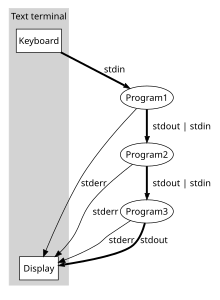
\includegraphics[scale=0.5]{sections/12_unix/images/Pipeline-notitle.svg.png}
\end{figure}

\paragraph{Tvorba skriptů}

\paragraph{Systémové proměnné}
\begin{center}
\begin{tabular}{|l|p{10cm}|}
\hline
\textbf{Proměnná} & \textbf{Popis} \\
\hline
\texttt{PATH} & Definuje cesty k adresářům, ve kterých jsou umístěny spustitelné soubory. \\
\hline
\texttt{HOME} & Cesta k domovskému adresáři aktuálně přihlášeného uživatele. \\
\hline
\texttt{USER} & Uživatelské jméno aktuálně přihlášeného uživatele. \\
\hline
\texttt{SHELL} & Cesta k interpretru příkazového řádku (shellu) pro aktuální uživatelskou relaci. \\
\hline
\texttt{PWD} & Aktuální pracovní adresář, tedy cesta ke složce, kde se uživatel momentálně nachází. \\
\hline
\texttt{LANG} & Určuje výchozí jazyk pro uživatelské rozhraní a programy. \\
\hline
\texttt{TERM} & Typ terminálu, který uživatel používá (např. xterm, rxvt, vt100). \\
\hline
\texttt{EDITOR} & Preferovaný textový editor pro úpravy textu. \\
\hline
\end{tabular}
\end{center}

\paragraph{Vrstvy}

\subsection{Meziprocesorová komunikace}
\paragraph{Semafor}
\paragraph{Sdílená paměť}

\subsection{Použití a popis služeb}
\paragraph{Telnet}
Telnet (Telecommunication Network) je označení protokolu používaného v počítačových sítích, který pomocí stejnojmenné aplikace umožňuje uživateli připojení ke vzdálenému počítači.
\begin{itemize}
    \item Protokol Telnet pracuje na aplikační vrstvě TCP/IP.
    \item Používá se v internetu pro realizaci spojení typu klient-server protokolem TCP, přičemž přenáší osmibitové znaky oběma směry (duplex).
    \item Serverová část standardně naslouchá na portu číslo 23.
    \item Součástí protokolu je vyjednání nastavení určitých voleb důležitých pro vzájemnou komunikaci.
\end{itemize}

\paragraph{SSH}
Secure Shell (SSH) je program a zároveň zabezpečený komunikační protokol v počítačových sítích, které používají TCP/IP.
\begin{itemize}
    \item SSH byl navržen jako náhrada za Telnet a další nezabezpečené shelly, které posílají heslo v nezabezpečené formě a umožňují tak jeho odposlechnutí při přenosu pomocí počítačové sítě.
    \item Šifrování přenášených dat, které SSH poskytuje, slouží k zabezpečení dat při přenosu přes nedůvěryhodnou síť, jako je například internet.
    \item SSH umožňuje bezpečnou komunikaci mezi dvěma počítači, která využívá pro zprostředkování přístupu k příkazovému řádku, kopírování souborů a také jakýkoliv obecný přenos dat.
    \item Zabezpečuje autentizaci obou účastníků komunikace, transparentní šifrování přenášených dat, zajištění jejich integrity a volitelnou bezdrátovou kompresi.
    \item Server standardně naslouchá na portu TCP/22.
\end{itemize}
\paragraph{FTP}
File Transfer Protocol (FTP) je protokol pro přenos souborů mezi počítači pomocí počítačové sítě.
\begin{itemize}
    \item Využívá protokol TCP/IP a může být používán nezávisle na použitém operačním systému.
    \item Používá se ke sdílení dat a správě účtu internetových stránek.
\end{itemize}

\paragraph{DNS}
Domain Name System (DNS) je systém doménových jmen, který je realizován servery DNS a protokolem stejného jména, kterým si vyměňují informace.
\begin{itemize}
    \item Jeho hlavním úkolem a příčinou vzniku jsou vzájemné převody doménových jmen a IP adres uzlů sítě.
    \item Dnes slouží jako distribuovaná databáze síťových informací.
    \item Servery DNS jsou organizovány hierarchicky, stejně jako jsou hierarchicky tvořeny názvy domén.
    \item Jména domén umožňují lepší orientaci lidem, adresy pro stroje jsou však vyjádřeny pomocí adres 32 bit (IPv4) nebo 128 bit (IPv6).
\end{itemize}

\paragraph{DHCP}
Dynamic Host Configuration Protocol (DHCP) je protokol z rodiny TCP/IP, který se používá pro automatické přidělení IP adres počítačům připojeným do počítačové sítě.

\begin{itemize}
    \item DHCP server přiděluje počítačům pomocí DHCP protokolu zejména IP adresu, masku sítě, výchozí bránu a adresu DNS serveru.
    \item Platnost přidělených údajů je omezená, proto je na počítači spuštěn DHCP klient, který jejich platnost prodlužuje.
\end{itemize}

\subsection{Virtualizace unixového prostředí na MS Windows}